\section{Задание 2: Решить задачи Коши}
    \subsection{Постановка задачи}
        Для заданных уравнений указать тип в простой форме. Найти общее реше-
        ние. Найти частное решение, удовлетворяющее заданным условиям. Построить
        график решения:

        \begin{enumerate}
            \item \( yy'' + y'^2 = 2e^y(1 + xy'); \quad y(0) = 0, ~ y'(0) = 0 \)
            
            \item \( y'' = \sqrt{1 + y'^2}; \quad y(1) = 1, ~ y'(1) = 0 \)
        \end{enumerate}

    \subsection{Решение}
        \begin{enumerate}
            \item \(
                \begin{cases}
                    yy'' + y'^2 = 2e^y(1 + xy')\\
                    y(0) = 0, ~ y'(0) = 0
                \end{cases}
            \) \label{eq2_1}

                \textit{Тип уравнения:}
                    Вполне интегрируемое уравнение.

                \textit{Общее решение:}
                    \( yy' = 2xe^y + C_1 \)

                \textit{Частное решение:}
                    \(-e^{-y}(y + 1) = x^2 - 1\)

                \begin{figure}[H]
                    \centering
                    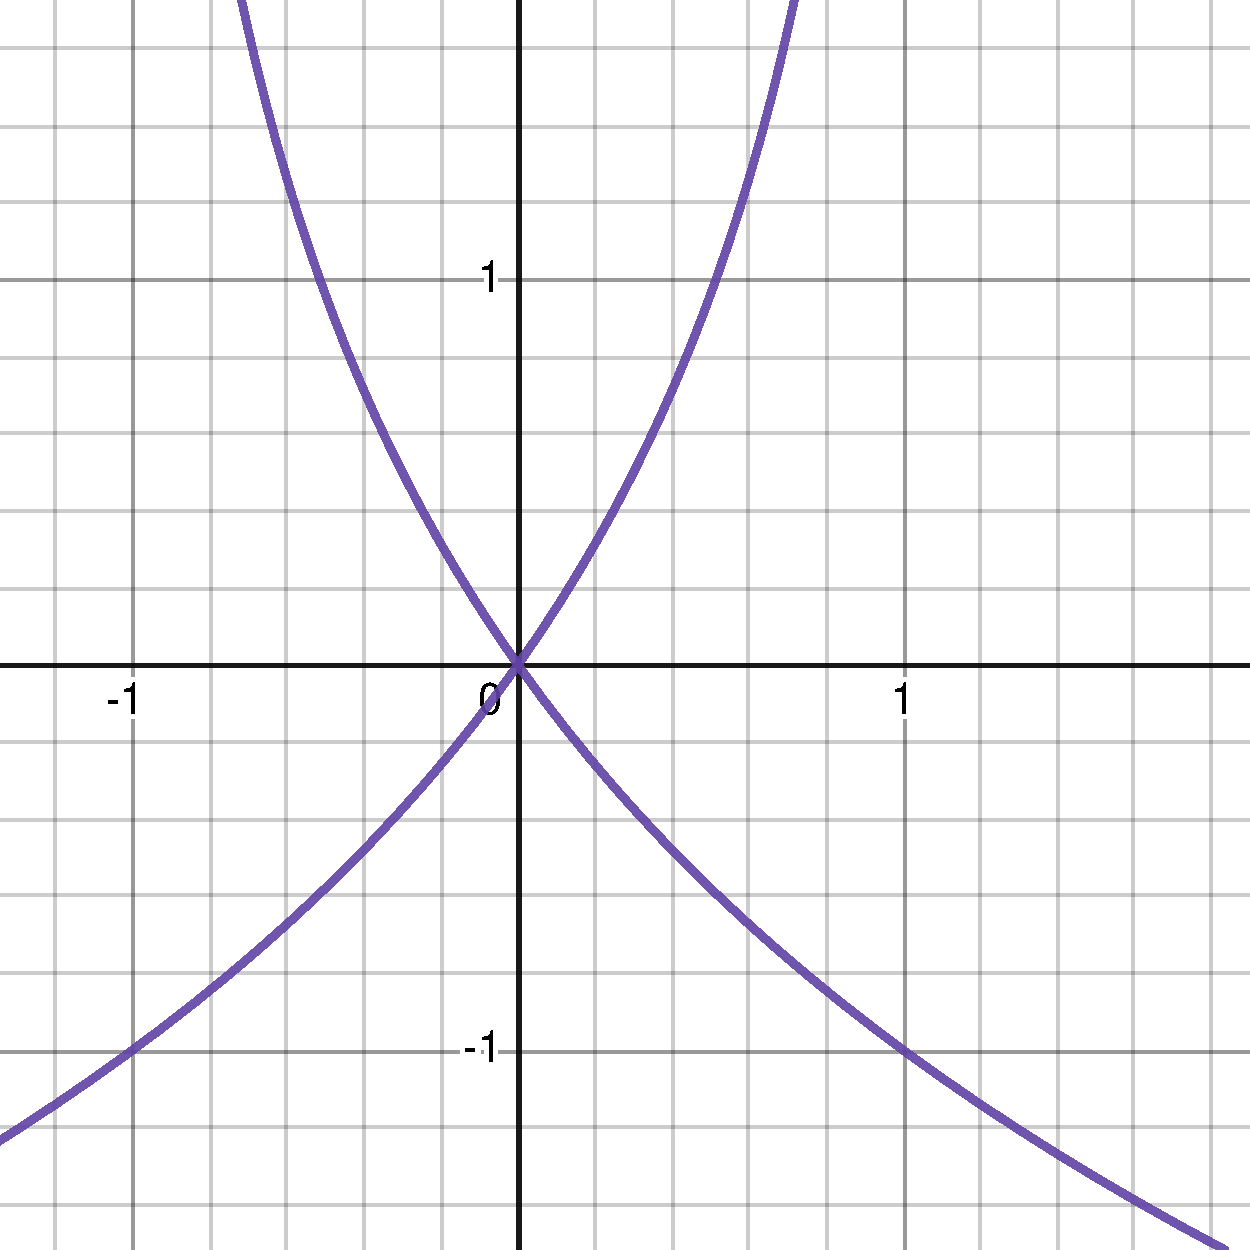
\includegraphics[width=7cm]{pics/2_1.pdf}
                    \caption{График решения уравнения (\ref{eq2_1})}
                \end{figure}


            \item \(
                \begin{cases}
                    y'' = \sqrt{1 + y'^2}\\
                    y(1) = 1, ~ y'(1) = 0
                \end{cases}  
            \) \label{eq2_2}

                \textit{Тип уравнения:}
                    Допускающее понижение порядка, несодержащее аргумент и искомую функцию.

                \textit{Общее решение:}
                    \( y = \cosh(x + C_1) + C_2 \)

                \textit{Частное решение:}
                    \( y = \cosh(x - 1) \)

                \begin{figure}[H]
                    \centering
                    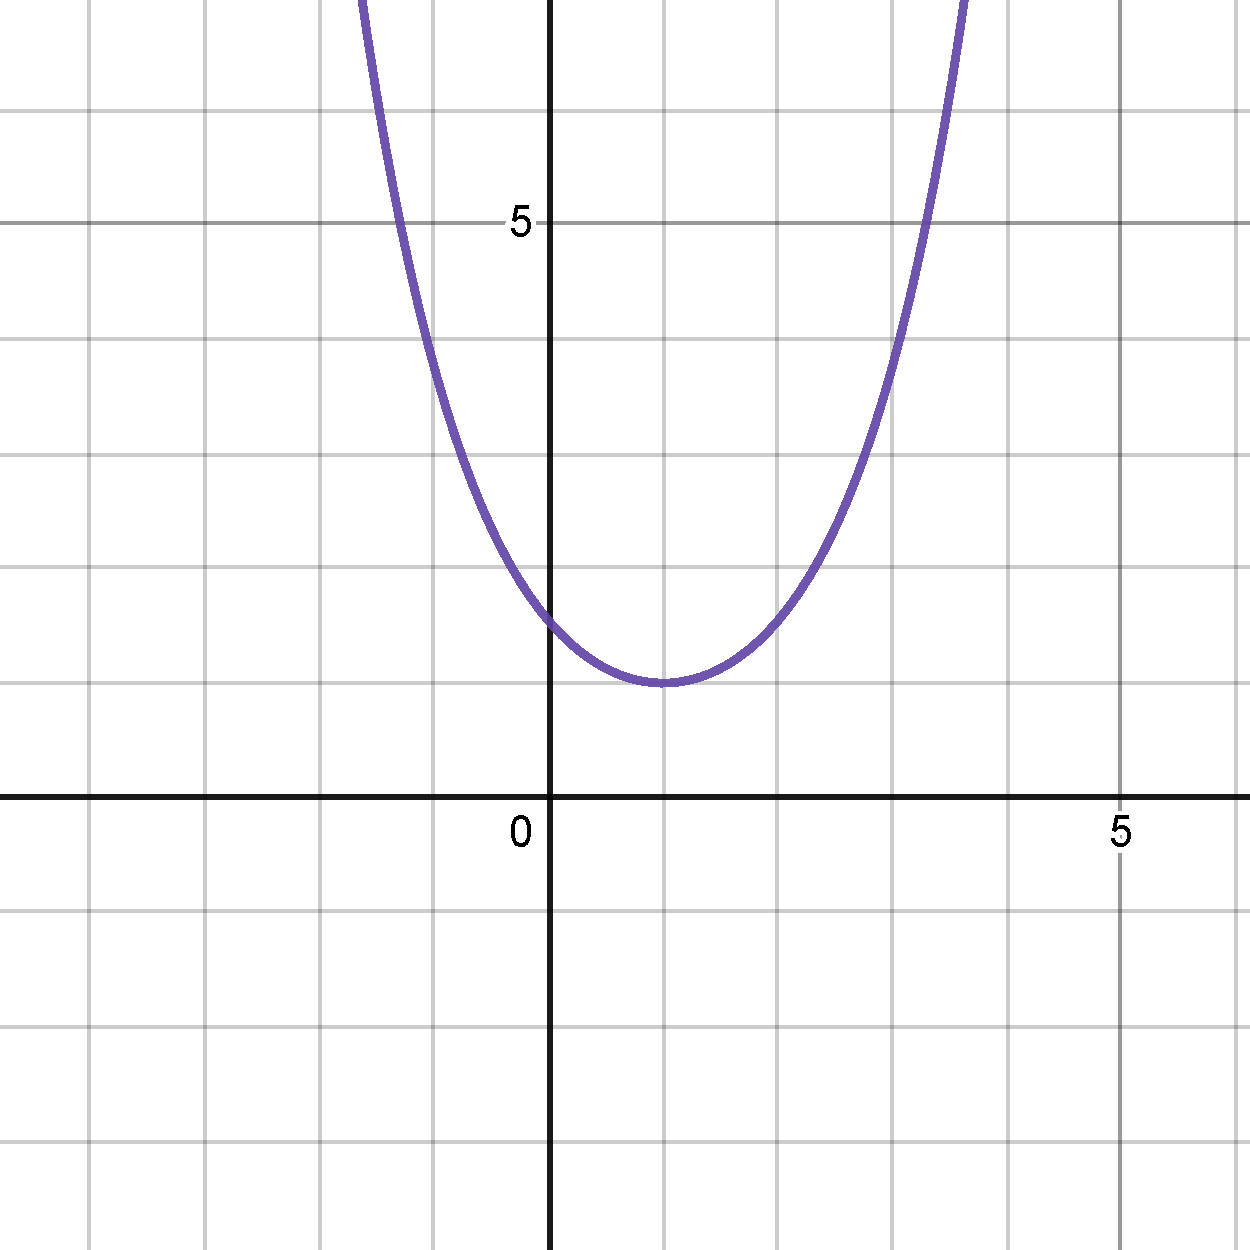
\includegraphics[width=7cm]{pics/2_2.pdf}
                    \caption{График решения уравнения (\ref{eq2_2})}
                \end{figure}
        \end{enumerate}